On place $650$ points à l'intérieur d'un disque de rayon $16$. Montrer
qu'il existe une couronne de rayon intérieur $2$ et de rayon extérieur $3$
(l'ensemble des points dont la distance à un centre donné est comprise entre
$2$ et $3$) qui contient $10$ de ces points.

\begin{center}
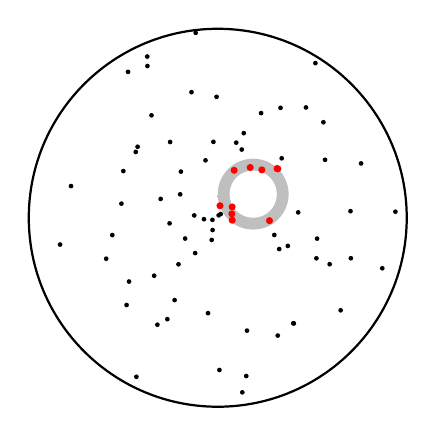
\begin{tikzpicture}[scale=.3]
  % Disque de rayon 16 (échelle 1/2)
  \draw[thick, fill=white] (0,0) circle (8);
  % Points au hasard dans le disque
  \foreach \i in {1,...,75} {
    \pgfmathsetmacro{\ta}{rand*360}
    \pgfmathsetmacro{\tr}{rand*8}
    \fill[black] ({\tr*cos(\ta)},{\tr*sin(\ta)}) circle (0.1);
  }
  % Couronne de rayons 2 et 3 (échelle 1/2)
  \fill[gray!50!white] (1.5,1) circle (1.5);
  \fill[white] (1.5,1) circle (1);
  % Dix points dans la couronne
  \foreach \i in {1,...,10} {
    \pgfmathsetmacro{\ta}{rand*360}
    \pgfmathsetmacro{\tr}{1.25 + 0.25*rand}
    \fill[red] ({1.5+\tr*cos(\ta)},{1+\tr*sin(\ta)}) circle (0.15);
  }
\end{tikzpicture}
\end{center}
